\documentclass[../main]{subfiles}

\begin{document}

\section{A ctbench use case}

This example covers a short yet practical example of ctbench usage. We want to
calculate the sum of a series of integers known at compile-time, using a type
template to store unsigned integer values at compile-time.

We will be comparing the compile-time performance of two implementations:

\begin{itemize}
\item one based on a recursive function template,
\item and one based on \cpp11 parameter pack expansion.
\end{itemize}

First we need to include \lstinline{utility} to instantiate our benchmark
according to the size parameter using \lstinline{std::make_index_sequence}, and
define the compile-time container type for an unsigned integer:

\begin{lstlisting}[language=C++]{}
#include <utility>

/// Compile-time std::size_t
template <std::size_t N> struct ct_uint_t {
  static constexpr std::size_t value = N;
};
\end{lstlisting}

The first version of the metaprogram is based on a recursive template function:

\begin{lstlisting}[language=C++]{}
/// Recursive compile-time sum implementation
template<typename ... Ts> constexpr auto sum();

template <> constexpr auto sum() { return ct_uint_t<0>{}; }
template <typename T> constexpr auto sum(T const &) { return T{}; }

template <typename T, typename... Ts>
constexpr auto sum(T const &, Ts const &...tl) {
  return ct_uint_t<T::value + decltype(sum(tl...))::value>{};
}
\end{lstlisting}

And the other version relies on \cpp11 parameter pack expansion:

\begin{lstlisting}[language=C++]{}
/// Expansion compile-time sum implementation
template<typename ... Ts> constexpr auto sum();

template <> constexpr auto sum() { return ct_uint_t<0>{}; }

template <typename... Ts> constexpr auto sum(Ts const &...) {
  return ct_uint_t<(Ts::value + ... + 0)>{};
}
\end{lstlisting}

Both versions share the same interface, and thus the same driver code as well.
The driver code takes care of scaling the benchmark according to
\lstinline{BENCHMARK_SIZE}, which is defined by \ctbench through the CMake API:

\begin{lstlisting}[language=C++]{}
// Driver code

template <typename = void> constexpr auto foo() {
  return []<std::size_t... Is>(std::index_sequence<Is...>) {
    return sum(ct_uint_t<Is>{}...);
  }
  (std::make_index_sequence<BENCHMARK_SIZE>{});
}

[[maybe_unused]] constexpr std::size_t result =
    decltype(foo())::value;
\end{lstlisting}

The CMake code needed to run the benchmarks is the following:

\begin{lstlisting}[language=CMake]{}
ctbench_add_benchmark(
  variadic_sum.expansion variadic_sum/expansion.cpp ${BENCHMARK_START}
  ${BENCHMARK_STOP} ${BENCHMARK_STEP} ${BENCHMARK_ITERATIONS})

ctbench_add_benchmark(
  variadic_sum.recursive variadic_sum/recursive.cpp ${BENCHMARK_START}
  ${BENCHMARK_STOP} ${BENCHMARK_STEP} ${BENCHMARK_ITERATIONS})
\end{lstlisting}

Then a graph target can be declared:

\begin{lstlisting}[language=CMake]{}
ctbench_add_graph(variadic_sum-compare-graph compare-all.json
                  variadic_sum.expansion variadic_sum.recursive)
\end{lstlisting}

with \lstinline{compare-all.json} containing the following:

\begin{lstlisting}[language=JSON]{}
{
  "plotter": "compare_by",
  "legend_title": "Timings",
  "x_label": "Benchmark size factor",
  "y_label": "Time (microsecond)",
  "draw_average": true,
  "demangle": false,
  "draw_points": false,
  "width": 800,
  "height": 400,
  "key_ptrs": ["/name", "/args/detail"],
  "value_ptr": "/dur",
  "plot_file_extensions": [".svg"]
}
\end{lstlisting}

This configuration file uses the \lstinline{compare_by} plotter to generate one
plot for each pair of elements designated by the JSON pointers in
\lstinline{key_ptrs}, namely \lstinline{/name} and \lstinline{/args/detail}. The
first pointer designates the LLVM timer name, and the second *may* refer to
metadata such a \cpp symbol, or a \cpp source filename. The \lstinline{demangle}
option may be used to demangle \cpp symbols using LLVM.

The result is a series of graphs, each one designating a particular timer event,
specific to a source or a symbol whenever it is possible (ie. whenever metadata
is present in the \lstinline{/args/detail} value of a timer event). Each graph
compares the evolution of these timer events in function of the benchmark size.

The graphs following were generated on a Lenovo T470 with an Intel i5 6300U and
8GB of RAM. The compiler is Clang
14.0.6, and [Pyperf](https://pyperf.readthedocs.io/en/latest/system.html) was
used to turn off CPU frequency scaling.

% TODO
% \begin{figure}[h]
% 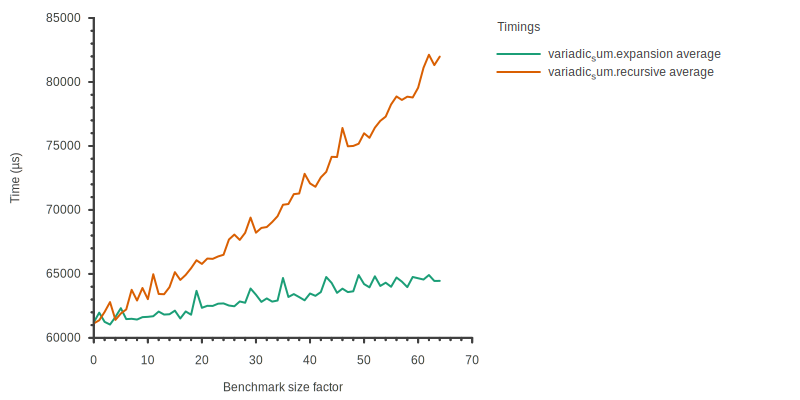
\includegraphics{docs/images/ExecuteCompiler.png}
% \caption{ExecuteCompiler}
% \end{figure}

The first timer we want to look at is ExecuteCompiler, which is the total
compilation time. Starting from there we can go down in the timer event
hierarchy to take a look at frontend and backend execution times.

% TODO
% \begin{figure}[h]
% 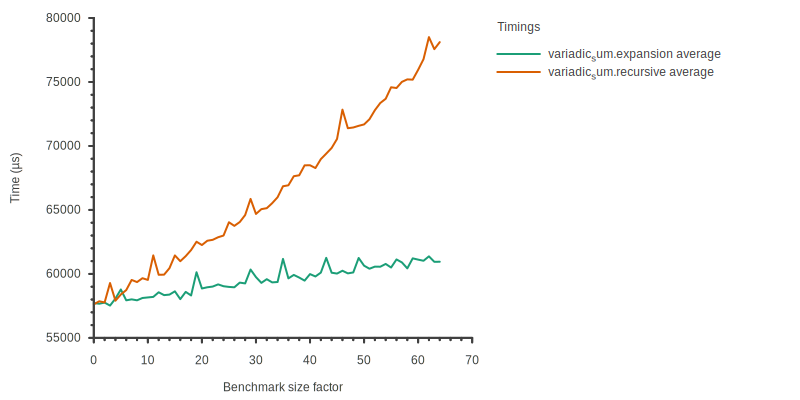
\includegraphics{docs/images/Total_Frontend.png}
% \caption{Total Frontend}
% \end{figure}

% TODO
% \begin{figure}[h]
% 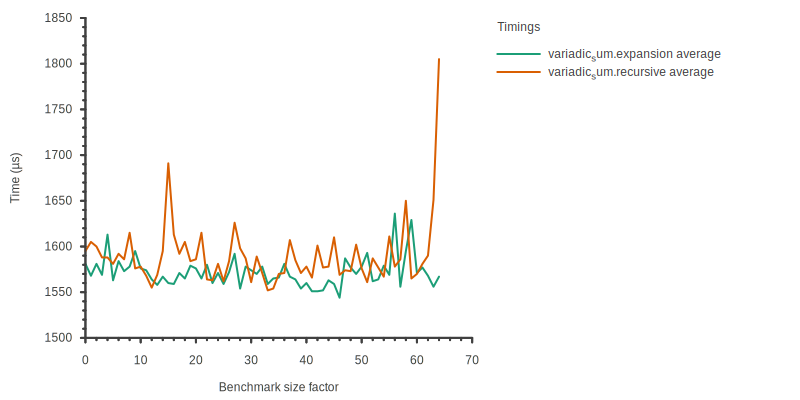
\includegraphics{docs/images/Total_Backend.png}
% \caption{Total Backend}
% \end{figure}

The backend is not being impacted here, supposedly because this is purely a
compile-time program, and the output program is empty. However this might not be
the case for all metaprograms, and metaprograms might have different impacts on
the backend as they may generate programs in different ways (ie. generate more
symbols, larger symbols, more data structures, etc.).

% TODO
% \begin{figure}[h]
% 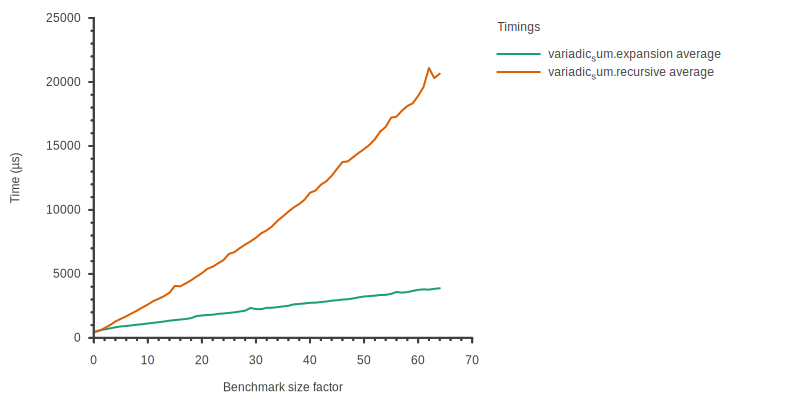
\includegraphics{docs/images/Total_InstantiateFunction.png}
% \caption{Total InstantiateFunction}
% \end{figure}

The Total Instantiate function timer is an interesting one as it explicitly
targets function instanciation time. Note that timers that are prefixed with
"Total" measure the total time spent in a timer section, regardless of the
specific symbol or source associated to its individual timer events.

% TODO
% \begin{figure}[h]
% 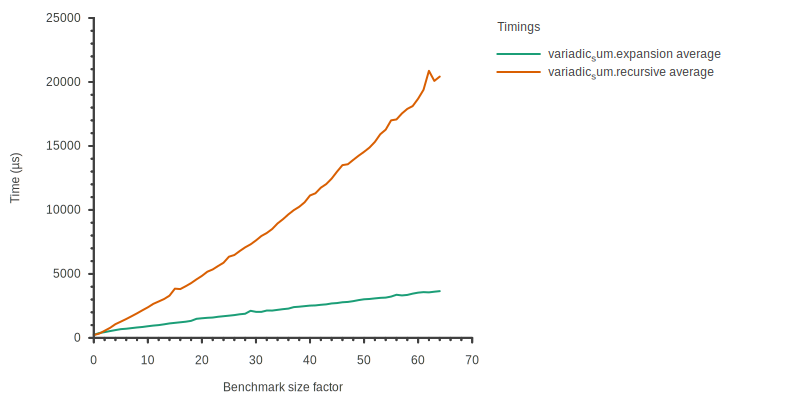
\includegraphics{docs/images/InstantiateFunction/foovoid.png}
% \caption{InstantiateFunction foovoid}
% \end{figure}

Finally, we can take a look at \lstinline{InstantiateFunction/foovoid.png} which
measures the InstantiateFunction event time specifically for
\lstinline{foo<void>()}, which is our driver template function. Using Perfetto
UI to look at the timer event hierarchy, we can validate that the timer event
for this specific symbol includes the InstantiateFunction time for all the
symbols that may be instantiated within this function.

This level of detail and granularity in the analysis of compile-time benchmarks
was never reached before, and may help us set good practices to improve the
compile-time performance of metaprograms.

\end{document}
